\section{Approach}\label{sec:approach}

\subsection{Architecture}\label{subsec:architecture}
This section covers the architecture, with which we achieved our best results, which are presented in Section \ref{sec:evaluation}. Our architecture is based on a published architecture~\cite{CTC} which achieved the best performance in the competition ICFHR 2014~\cite{icfhr_competition}.

The task of digit string recognition poses several challenges across different machine learning disciplines.
On the one hand, the input image is a high-dimensional tensor (after resizing $120\times50\times3$).
As a consequence, the input will have a low information density and considerable amount of noise.
A proven neural network architecture class for processing images are convolutional neural networks (CNN).
More specifically, we employ a smaller variant of the Residual Network (ResNet)~\cite{ResNet} architecture.
See Fig.~\ref{fig:resblock} for a detailed view of our implementation of the residual architecture.
After every convolutional layer we performed batch normalization~\cite{batchnorm} to prevent internal covariance shift and accelerate training.
This first step in our architecture can be seen as an \emph{encoder}, mapping the input image to a 3 dimensional tensor with lower spatial dimensions ($15 \times 6$) but more channels (512).

We then interpret the output as a sequence along the horizontal axis.
For simplicity we have designed the horizontal output dimension of the encoder to be equal to the maximal sequence length.
In this case every column matrix (of size $6 \times 512$ represents one sequence element).
If this is not possible or the sequence length should be variable without changing the encoder, a linear projection can be used to increase or decrease the horizontal dimension.

The remaining task is to decode this tensor by labeling every element of the sequence with a digit or blank.
We output scores for every digit and blank for each element in the sequence.
The output dimensionality of every label is therefore 11.
As described in Section \ref{subsec:rnn}, vanilla RNNs suffer from the vanishing gradient problem.
We therefore use long short term memory (LSTM)~\cite{LSTM}, which mitigate this issue.
LSTMs can be stacked by using the output of the previous layer as input to the next layer.
We use two layer LSTMs to allow the network to learn a more complex function.
In addition we use bidirectional LSTMs (BiLSTM), which are independently applied to the original sequence and the reversed sequence and combine their outputs by addition.
Our BiLSTM outputs a 100-d vector at every time step.
Finally a linear layer is used to reduce this dimension to 11.
During training we use log-softmax to prepare the output for calculation of the CTC-Loss.
When inferring labels we select the element with the highest output using the argmax operator at each time step.
The full architecture is shown in Fig.~\ref{fig:architecture}.

\begin{figure}
    \begin{center}
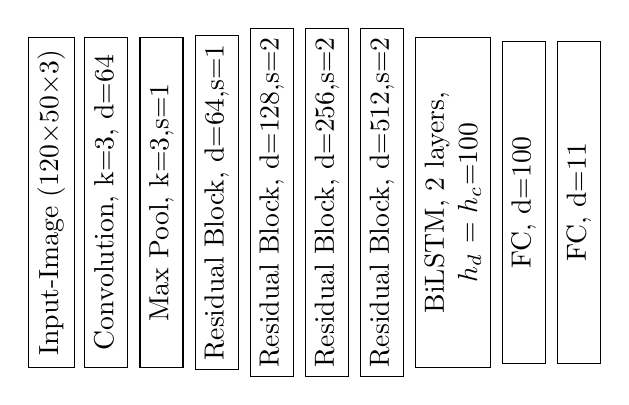
\begin{tikzpicture}
    \node[rectangle,minimum width=4.2cm,draw,rotate=90] at (0,2.1) (input) {Input-Image (120$\times$50$\times$3)};
    \node[rectangle,minimum width=4.2cm,draw,rotate=90] at (0.7,2.1) (conv1) {Convolution, k=3, d=64};
    \node[rectangle,minimum width=4.2cm,draw,rotate=90] at (1.4,2.1) (pool1) {Max Pool, k=3,s=1};
    \node[rectangle,minimum width=4.2cm,draw,rotate=90] at (2.1,2.1) (res1) {Residual Block, d=64,s=1};
    \node[rectangle,minimum width=4.2cm,draw,rotate=90] at (2.8,2.1) (res2) {Residual Block, d=128,s=2};
    \node[rectangle,minimum width=4.2cm,draw,rotate=90] at (3.5,2.1) (res3) {Residual Block, d=256,s=2};
    \node[rectangle,minimum width=4.2cm,draw,rotate=90] at (4.2,2.1) (res4) {Residual Block, d=512,s=2};
    %\node[rectangle,minimum width=2.1cm,draw,rotate=90] at (5.25,1.05) (reverse) {reverse};
    \node[rectangle,minimum width=4.2cm,draw,rotate=90,align=center] at (5.1,2.1) (bilstm) {BiLSTM, 2 layers, \\ $\text{h}_d$ = $\text{h}_c$=100};
    \node[rectangle,minimum width=4.1cm,draw,rotate=90] at (6,2.1) (fc1) {FC, d=100};
    \node[rectangle,minimum width=4.1cm,draw,rotate=90] at (6.7,2.1) (fc2) {FC, d=11};
\end{tikzpicture}
\caption{\it Schematic of our architecture. Dropouts and batch normalizations are omitted for brevity.}\label{fig:architecture}
\end{center}
\end{figure}
\begin{figure}
    \begin{center}
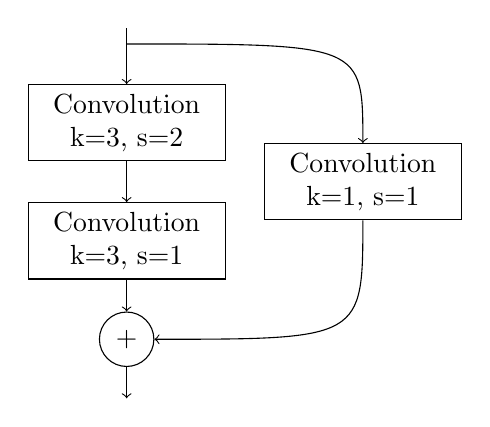
\begin{tikzpicture}
    \node[rectangle, minimum width=2.5cm,draw,align=center] at (0,-1) (conv1) {Convolution\\ k=3, s=2};
    \node[rectangle, minimum width=2.5cm,draw,align=center] at (0,-2.5) (conv2) {Convolution\\ k=3, s=1};
    \node[rectangle, minimum width=2.5cm,draw,align=center] at (3,-1.75) (resconv) {Convolution\\ k=1, s=1};
    \node[circle,draw,align=center] at (0,-3.75) (add) {$+$};
    \draw[->] (0,0.2) -- (conv1);
    \draw[->] (conv1) -- (conv2);
    \draw[->] (0,0) .. controls (3,0) .. (resconv);
    \draw[->] (conv2) -- (add);
    \draw[->] (resconv) .. controls (3,-3.75) .. (add);
    \draw[->] (add) -- (0,-4.5);
\end{tikzpicture}
\caption{\it Schematics of a residual block in our architecture. If the output dimension does not change (as in our first residual block, the linear mapping in the residual path is not required and therefore omitted. Furthermore does the first residual block use a stride of 1 instead of 2.}\label{fig:resblock}
\end{center}
\end{figure}
\subsection{Training}\label{subsec:training}

We divided our training in epochs.
In each epoch we observe every training sample once.
Each sample is randomly manipulated by different data augmentation methods as described in Section \ref{Datasets}.
We normalized each sample by channel-wise whitening (subtracting dataset mean color value and dividing by dataset variance).
The Adam~\cite{Adam} is used to minimize the CTC loss per batch.
We found a batch-size of 32 to deliver the best results.
Higher batch-sizes resulted into very slow learning, due to seldom updates, while lower batch-sizes did had less parallelization on GPU and where therefore slower to compute.
Increasing the step size when using higher batch-sizes did not speed up training either.
We suspect that the loss function surface is shaped in a way, such that higher variance gradient descent (as achieved by lower batch-sizes) results in faster convergence.

For hyper-parameter optimization we split our training data in a training and validation dataset, whereby 80\% of the training data is used for training and the rest is only used to evaluate the model performance.
